
\section{PROTOTYPE}
%; it turns index fingertip into a touchpad, by attaching the sensing plate on the user' index fingernail and the magnet on the thumbnail (Figure \ref{fig:firstFigure}). 
FingerPad is a pair of nail-mounted devices comprising of a thin (1mm) magnetic sensing plate, and a plate of ferromagnet. 
The sensing plate includes a 3x3 Winson WSH138 Hall sensor grid (Figure \ref{fig:hallDevice}a), and each sensor is separated to each other by 2mm, which suggests an area of 12(W) mm x 12(H) mm. 
Each sensor element detects both N- and S-polar magnetic field intensities in a range from 0 to 200 Gauss on a 1024-point scale. 
An Arduino board with an ATmega32U4 microprocessor is used to bridge the sensing plate with the computer.
According to the magnetic strength captured by the plate, FingerPad approximates the magnet's position, transforms the position to the finger-pad coordinate defined through user calibration (see  \emph{Tracking} and  \emph{User calibration}), and sends to the applications. 

\begin{figure}
\begin{center}
  \begin{tabular}{@{\hspace{0.1cm}}c}
		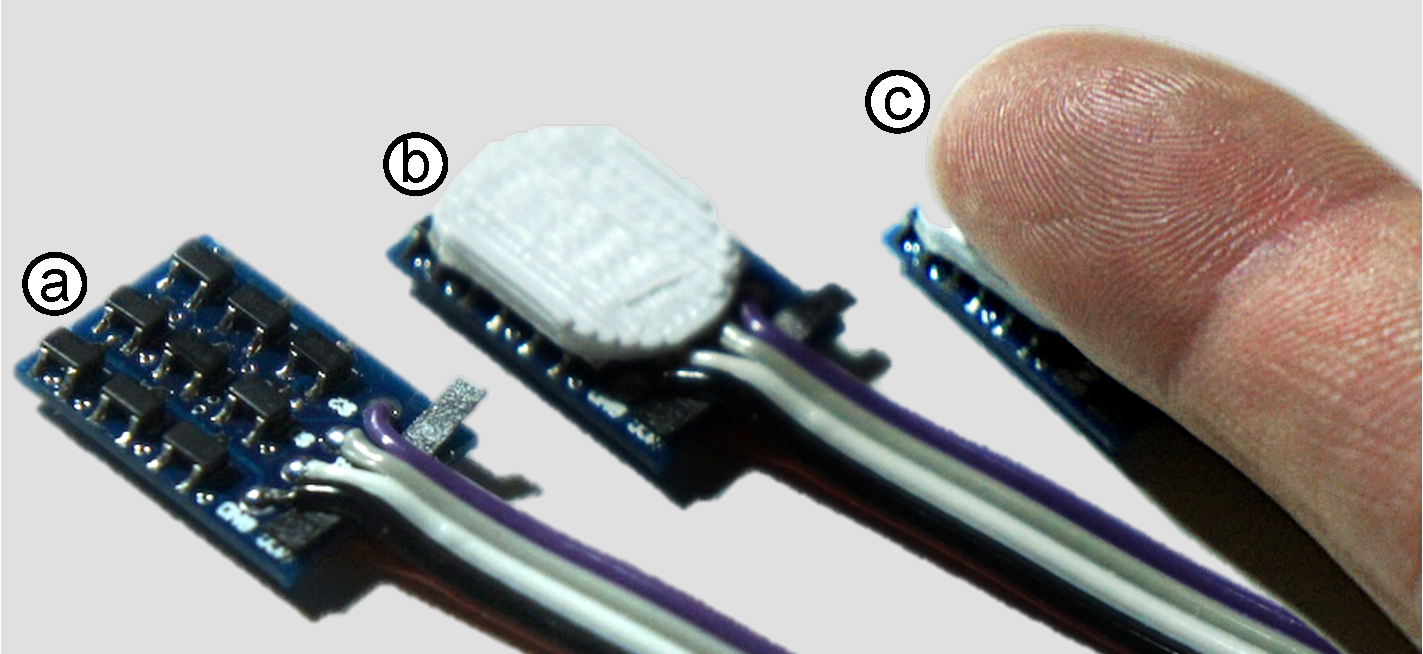
\includegraphics[width=1\linewidth]{hallDevice}
   \end{tabular}
\caption{(a) The 3x3 hall sensor grid, and (b) a nail-shape plate with a curve surface (c) suggesting fitness to the natural nail. }
\label{fig:hallDevice}
\end{center}
\end{figure}

\begin{figure}
\begin{center}
  \begin{tabular}{@{\hspace{0.1cm}}c}
		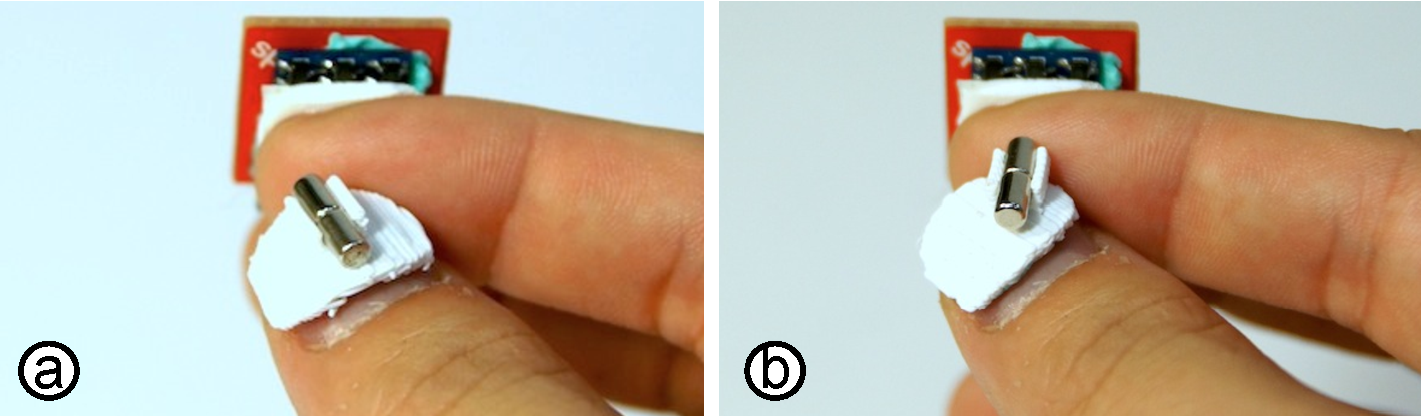
\includegraphics[width=1\linewidth]{magnetHolder3}
   \end{tabular}
\caption{The magnet holder grips the magnet at certain orientation. 
(a) The first design of the magnet holder. (b) we push the magnet orientation 30 degree to the right, accommodating to the bio-mechanism of the index and thumb fingers.}
\label{fig:magnetHolder}
\end{center}
\end{figure}

To attach the sensor plate firmly on the nail, we use a 3D printer to craft a nail piece that suggests a nail-fit curve surface. 
As shown in Figure \ref{fig:hallDevice}b, the sensor plate, gluing with the nail piece, is further glued on the user's nail using a twin adhesive tape. 
By gluing, we help users envision the future nail devices akin to the use of the artificial nails.
We put on the prototype on the user's index fingernail in a way that the wires would not affect the finger motor space.

We create another nail piece that holds the magnet and fixates the magnet orientation. 
The principle to place the magnet is to allow the polar orientation of the magnet in parallel with the normal of the sensor grid when users placing the thumb on the center of the index fingertip. 
Figure \ref{fig:magnetHolder}a shows our first design. 
To adapt the bio-mechanism of the thumb and index finger, we improve the design by moving the magnet orientation 30 degree to the right (Figure \ref{fig:magnetHolder}b). 
%This way, we improve and maximize the tracking range.

The magnet we used is a 2mm disk x 8mm strong ferromagnet, which allows for effectively sensing within 2.1cm by our sensor plate.
% allowing for the magnetic field remotely visible to the hall sensor plate on the index fingernail.
Note that this effective distance can be further extended by using more sensitive magnetism sensors, such as magnetometers \cite{Ashbrook:2011}.
% and maximizing the user envisioning the future device.

%This instrument is not suitable for measuring weak fields, such as the geomagnetic field.

%\subsection{Future device}
%show photo of skin-thin hall sensor grid. 



\subsection{Tracking}
We define a cartesian coordinate for the sensor-grid coordinate. 
For the 3 by 3 sensor grid, the sensor at the lower left corner is set as the coordinate origin. 
We approximate the magnet position in the sensor-grid coordinate using bilinear weighting according to the magnetic strength read by each hall sensor. 
Because the read magnetic field strength is in fact a mix of quadratic and cubic attenuation, this approach can only approximate the magnet position. 
We further regulate the positioning result in the \emph{User Calibration} section.

To improve the positioning, two strategies are applied. 
First, the polar of the magnet is placed in parallel with the normal of the sensor grid as shown in Figure \ref{fig:magnetHolder}b.
Second, we exclude the opposite polar values read by the sensors. 
When users tap on the edges of the index fingertip (e.g., the tip or bottom areas), 
the magnet orientation may deviate from the normals of the sensors, which causes some sensors read the opposite polar values. %and confusing the positioning.

%Third, we restraint the sensing area to only around the 

% As a result, we can reliably compute the magnet position in the sensor-grid coordinate.

\subsection{User calibration}
The purpose of user calibration is to regulate the 2D positions computed in \emph{Tracking}, to the finger-pad coordinate in the index fingertip.
%, to (2) maximize the use of real estate in the user's fingertip.
To account for the non-linear mappings between the sensor-grid and the finger-pad coordinates, we divide the finger-pad coordinate into multiple sub-coordinates, and approximate the nonlinearity by computing homographic transformation between each sub-coordinate and the sensor-grid coordinate. 
%This piece-wise approximation allows us to reduce the transformation errors.

\begin{figure}
\begin{center}
  \begin{tabular}{@{\hspace{0.1cm}}c}
		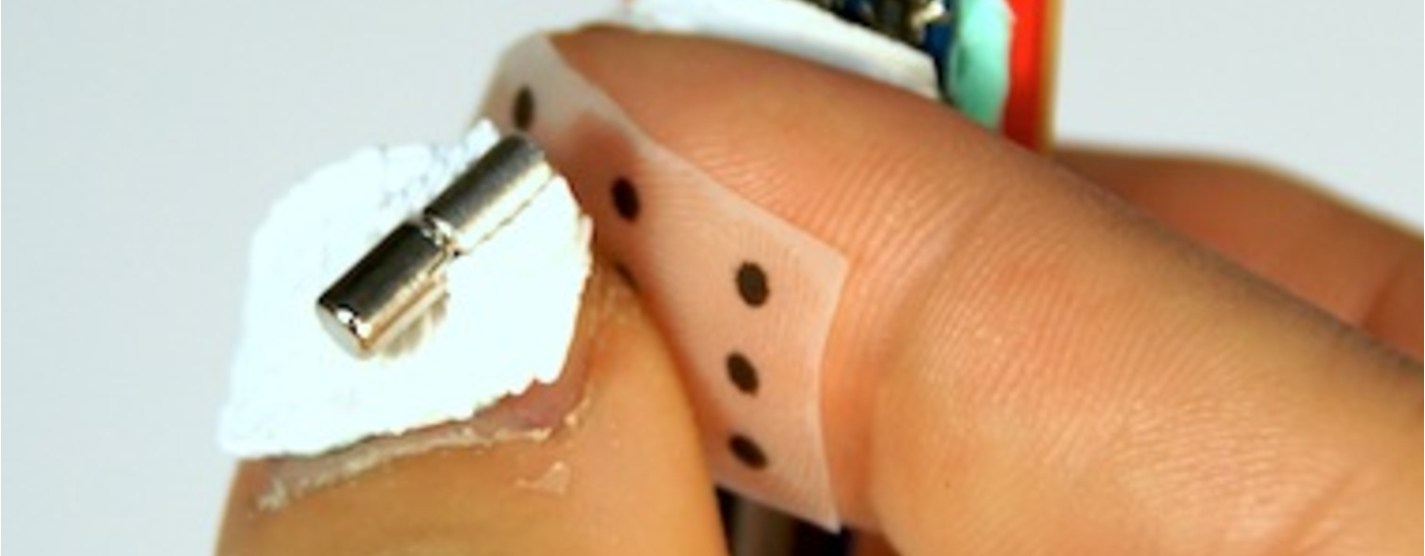
\includegraphics[width=1\linewidth]{userCalib3}\\
   \end{tabular}
\caption{To guide the calibration process, we stick a translucent dot pattern on the index fingertip, that helps to obtain good homographic transformations.}
%\caption{The participant's fingertip is sticked with a translucent pattern for touch positioning. (a) Translucent dot patterns in different fingertip sizes. (b) Edges of the pattern is cut open in order to fit curve surface of fingertip.}
\label{fig:userCalib}
\end{center}
\end{figure}

Typically, a homographic transformation can be determined by more than 4 pairwise correspondent points. 
To guide the calibration process, we stick a translucent dot pattern on the index fingertip. 
The dots are separated by 4mm in a Cartesian coordinate, and the 3 by 3 dot pattern suggests a normal size of the fingertip. 
We stick the pattern on the index fingertip area, as shown in Figure \ref{fig:userCalib}. 
The 9 pairs of the correspondent points from calibration process are then used to compute the homographic transformation for each of the four sub-coordinates. 
As long as the magnet orientation correctly positioned, the calibration configuration can adapt well to fingers with different sizes and thickness.
% only if the magnetic field is still sufficiently visible.

%Because the nail is typically smaller than the finger pad, when tapping to the edges of the index finger pad, the magnet may point outside of the proper range of the sensor grid, and affect the positioning result.

%We use the same translucent stick but in different dot pattern, to guide the user through calibration.
%The dots, separating by 2mm, form a cartesian coordinate (Figure \ref{fig:userCalib}a); a 3 by 4 dot pattern suggests a normal (need detail) finger size. (how to deal with different finger size?)
%To accommodate different finger sizes, we increase the pattern size by adding more dots, which increases user efforts in calibration but minimizes the positioning errors. 
%As in pilot study, we glue the pattern on the user's index fingertip in a way that keeps the bezel area clean (Figure \ref{fig:userCalib}b).
%During calibration, we instruct the user to press each dot and bezel button once with the thumb tip. Our system records the positions computed from \emph{Tracking} and the dot positions in the finger coordinate.


\subsection{Land-on detection}
Although the hall sensor plate can detect hover state (e.g., the thumb is in the proximity to the index fingertip) according to the strength of the magnetic field, it is hard to determine when the user's thumb landing-on the index fingertip.
To detect land-on, we add an accelerometer to the hall sensor plate to detect the impact of the finger contacts.
For the detail, we compute the derivative in the X, Y, and Z-axes, respectively, by using a sliding window. 
Through monitoring the values in the sliding window, a candidate for land-on can be found when a positive derivate is followed by a negative derivative.
A land-on action is only reported, when the thumb is found within the hover range at the same time.
After land-on, touch interactions performed by the user can be recognized, until the thumb is out of the hover range.

\subsection{Flick selection}
We propose the flick selection, as shown in Figure \ref{fig:flickSelection}.
Moving the cursor over a target, the user commits a selection by taking off the thumb up.
Upon exit of the hover state, we remove the cursor movement in the last 180 milliseconds (determined from a pilot testing) to eliminate the unwanted cursor movement. The last cursor position is used to determine the selection. 
The side effect of the flick selection is that the user may see the unwanted cursor movement before the thumb exits the hover state.
Nevertheless, the users can understand it and it won't affect users' performance.  

%Even though they understood these extra traces would not be counted in the selection process, the participants reported in our user study that they felt uncomfortable for this effect.

%\subsection{Choice of magnets}
%show a series of magnets, their 3d magnetic field shape, and the heights suggested.
%Rationalize why we choose the magnet in the prototype.


%While the Tracking reports 2d positions which are relative yet irregular (e.g., non-uniform), we regulate these positions by including manual calibration.

%To guide the user through calibration, we print a dot grid pattern on a translucent adhesive film. 


%\subsection{Evaluation}
%report errors with fewer calibration dots. using 2mm dot as ground truth.

\section{APPLICATION}
%To demonstrate FingerPad as an input method for the glass display, we implenment a glass interface using the LCD screen, as shown in Figure \ref{fig:glassUI}. 
Based on the touchpad functions provided by our prototype, we implement the touch cursor, gesture input, and stroke input functions to prove the capability of the FingerPad. 
The implemented application is the same as described in the \emph{SCENARIO} section.
 In the touch cursor function, a user can perform a long press to enter the cursor mode which reveals the cursor on the display (e.g., glass interface). 
 By moving the thumb on the index fingertip, the user can freely move the cursor. 
 Through the flick selection, the user can commit a selection on the menu. 
 For the gesture input, we also provide swipe and circling gestures. 
 In a page view, the user can swipe to left or right to enter the next or previous page. 
 In a list view, the user can perform clockwise or counter-clockwise circling gesture to scroll down or up through the list. 
 In stroke input, we adapt the unistroke recognizer \cite{Wobbrock:2007} for our numeric input, which allows users to write the password or phone numbers. 

\begin{figure}
\begin{center}
  \begin{tabular}{@{\hspace{0.1cm}}c}
		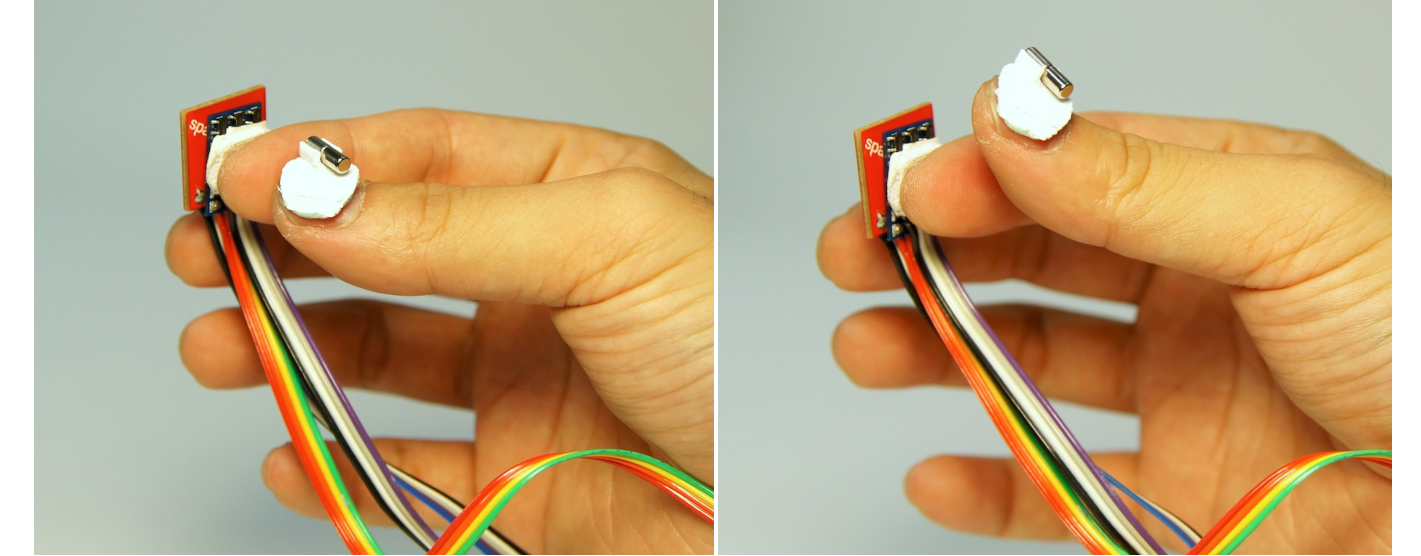
\includegraphics[width=1\linewidth]{flickSelection2}\\
   \end{tabular}
\caption{The user commits a selection by flicking the thumb up.}
\label{fig:flickSelection}
\end{center}
\end{figure}

